% -*- mode: LaTeX; compile-command: "pdflatex what-does-CS-look-like.tex" -*-

\documentclass[xcolor={usenames,dvipsnames,svgnames,table},12pt]{beamer}

\mode<presentation>
{
  \usetheme{default}                          % use a default (plain) theme

  \setbeamertemplate{navigation symbols}{}    % don't show navigation
                                              % buttons along the
                                              % bottom
  \setbeamerfont{normal text}{family=\sffamily}

%  \setbeamertemplate{footline}[frame number]

  \AtBeginSection[]
  {
    \begin{frame}<beamer>
      \frametitle{}
      \begin{center}
        {\Huge \insertsectionhead}

        % \vspace{0.25in}
        % \includegraphics[width=2in]{\secimage}
      \end{center}
    \end{frame}
  }
}

\newenvironment{xframe}[1][]
  {\begin{frame}[fragile,environment=xframe,#1]}
  {\end{frame}}

% uncomment me to get 4 slides per page for printing
% \usepackage{pgfpages}
% \pgfpagesuselayout{4 on 1}[uspaper, border shrink=5mm]

% \setbeameroption{show only notes}

\usepackage[english]{babel}
\usepackage[T1]{fontenc}
\usepackage{graphicx}
\graphicspath{{images/}}

\usepackage{ulem}
\usepackage{url}
\usepackage{fancyvrb}

% \title{Computer Science History}
% \date{}
% \author{Dr.\ Brent Yorgey}

%%%%%%%%%%%%%%%%%%%%%%%%%%%%%%%%%%%%%%%%%%%%%%%%%%%%%%%%%%%%%%%%%%%

\begin{document}

\begin{frame}{}
  \begin{center}
    {\Large Guess the computer scientist!}
  \end{center}
\end{frame}

\begin{frame}{}
  \begin{center}
    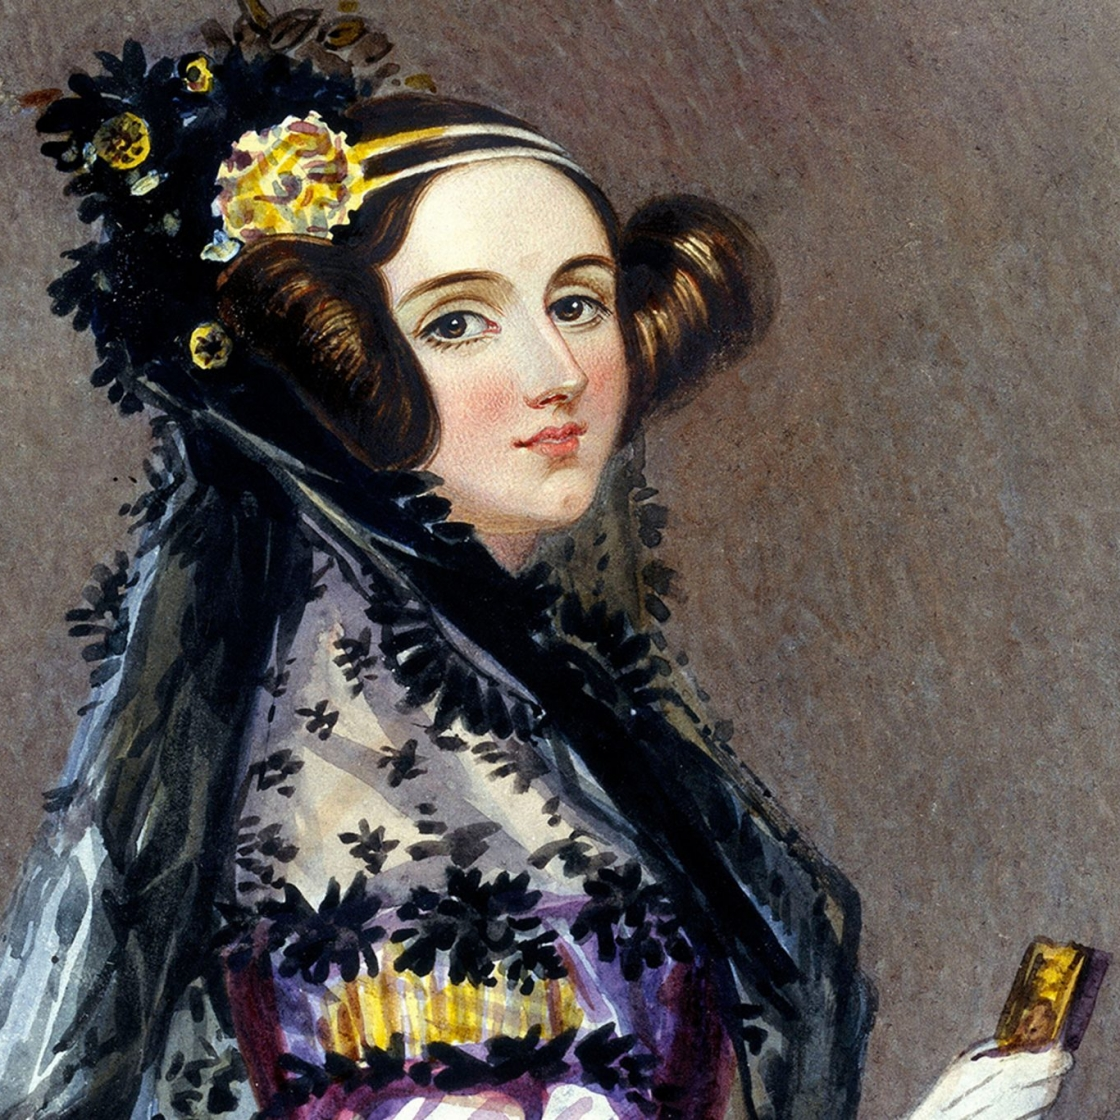
\includegraphics[height=2in]{ada-lovelace.jpeg} \quad
    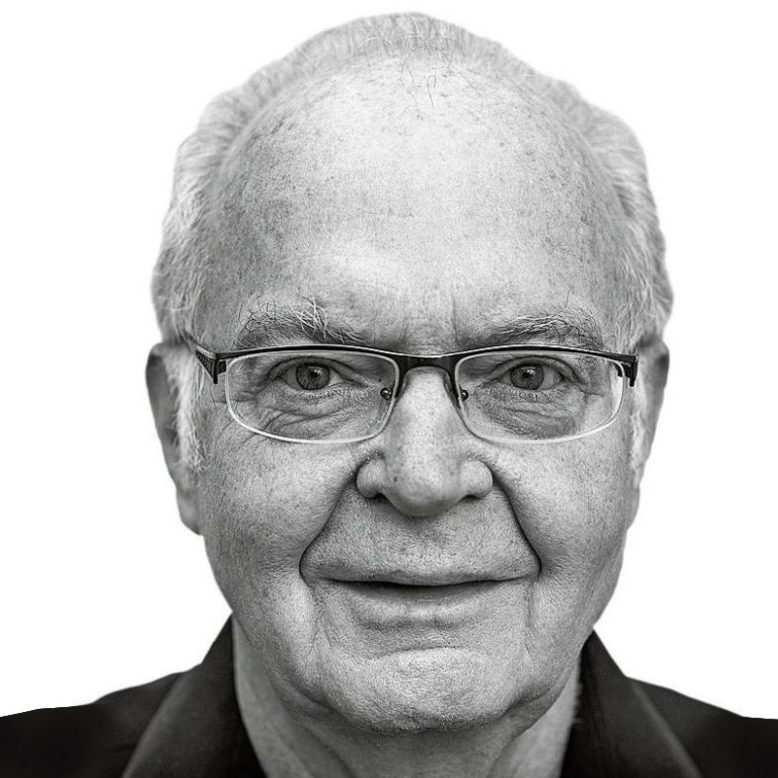
\includegraphics[height=2in]{donald-knuth.jpeg}
  \end{center}
\end{frame}

\begin{frame}{}
  \begin{center}
    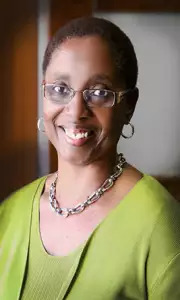
\includegraphics[height=2in]{valerie-taylor.jpg} \quad
    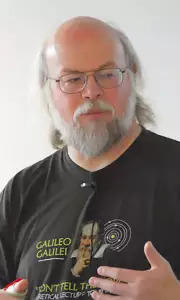
\includegraphics[height=2in]{james-gosling.jpg}
  \end{center}
  % Valerie Taylor: Director of the Mathematics and Computer Science
  % Division at Argonne National Laboratory. HPC.
  % James Gosling: lead designer of Java
\end{frame}

\begin{frame}{}
  \begin{center}
    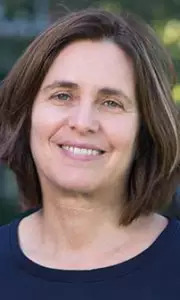
\includegraphics[height=2in]{shafi-goldwasser.jpg} \quad
    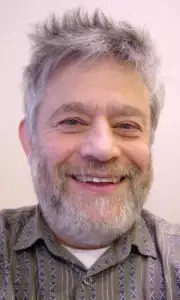
\includegraphics[height=2in]{manuel-blum.jpg}
  \end{center}
  % Shafi Goldwasser
  % Manuel Blum
  % Complexity theory, applications to security
\end{frame}

\begin{frame}{}
  \begin{center}
    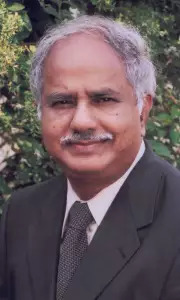
\includegraphics[height=2in]{dabbala-reddy.jpg} \quad
    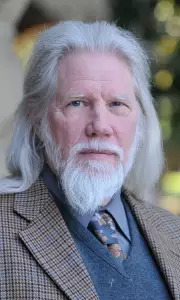
\includegraphics[height=2in]{whitfield-diffie.jpg}
  \end{center}
  % Raj Reddy: Turing Award, early pioneer of AI.
  % Whitfield Diffie: public key cryptography
\end{frame}

\begin{frame}{}
  \begin{center}
    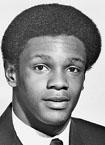
\includegraphics[height=1.5in]{ellis_skip_young.jpeg} \quad
    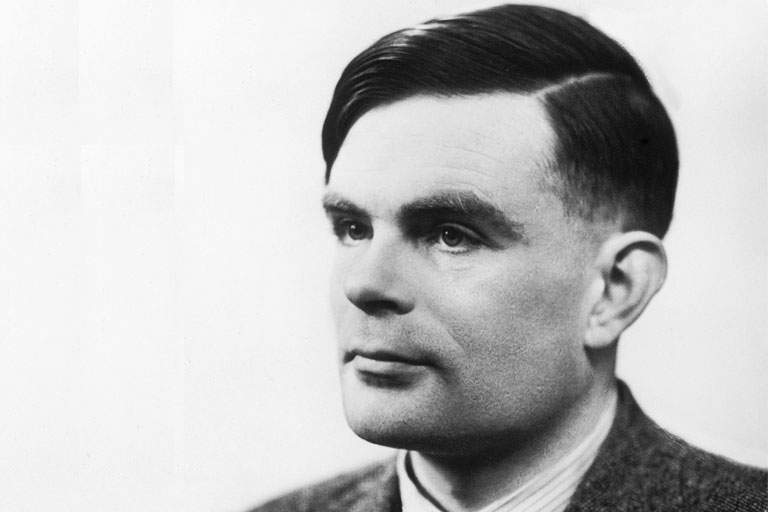
\includegraphics[height=1.5in]{Alan-Turing.jpeg}
  \end{center}
  % Skip Ellis: first black man to get a PhD in computer science,
  %   1969.  Foundational work in collaborative computing systems,
  %   behind e.g. Googld Docs.
  % Alan Turing:
\end{frame}

\begin{frame}{}
  \begin{center}
    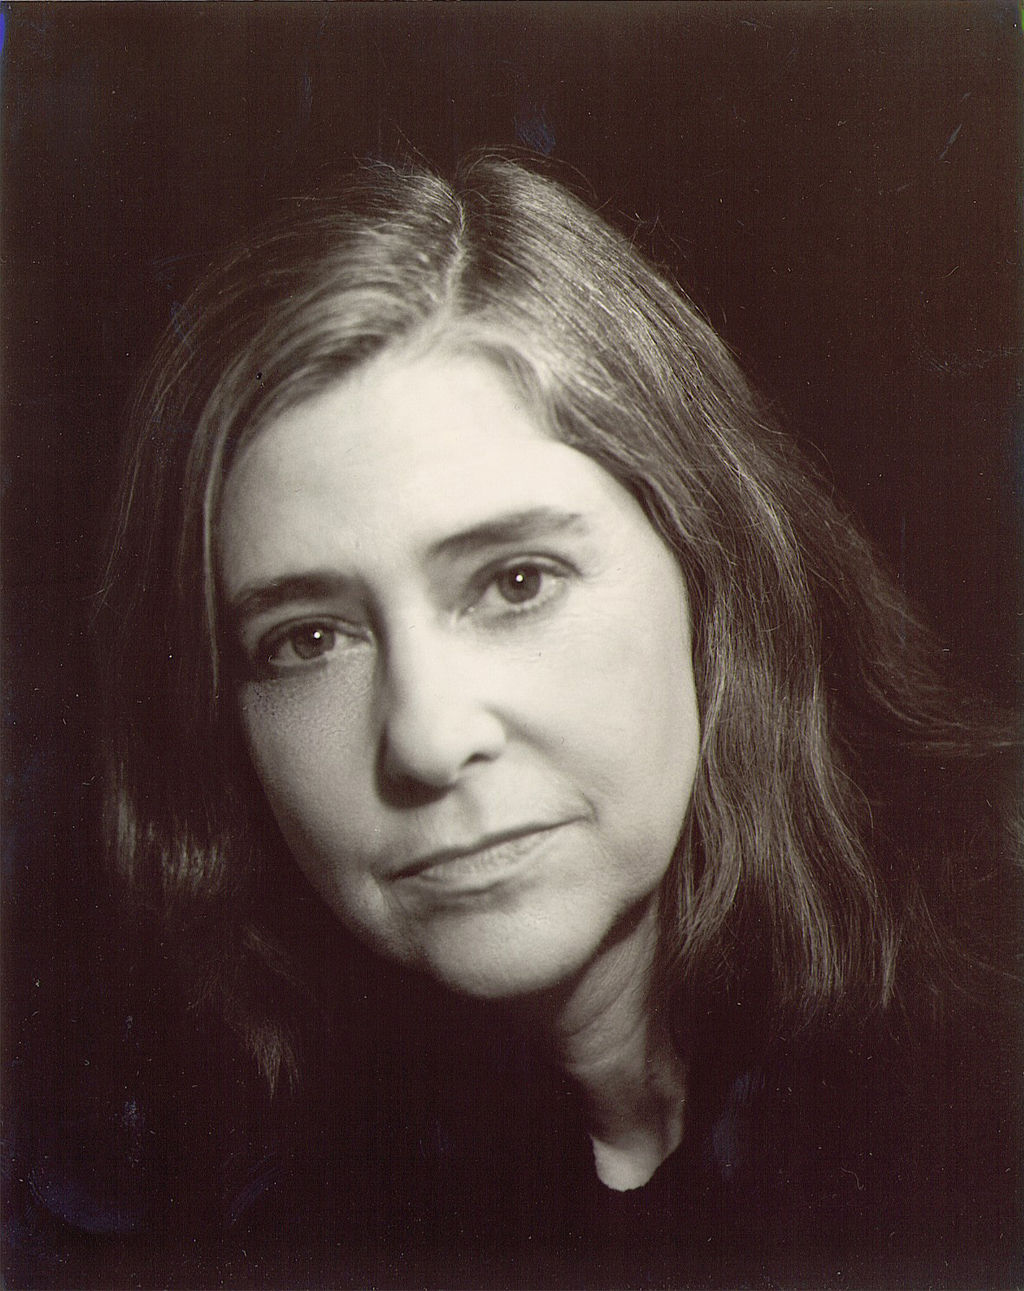
\includegraphics[height=2in]{Margaret-Hamilton.jpeg} \quad
    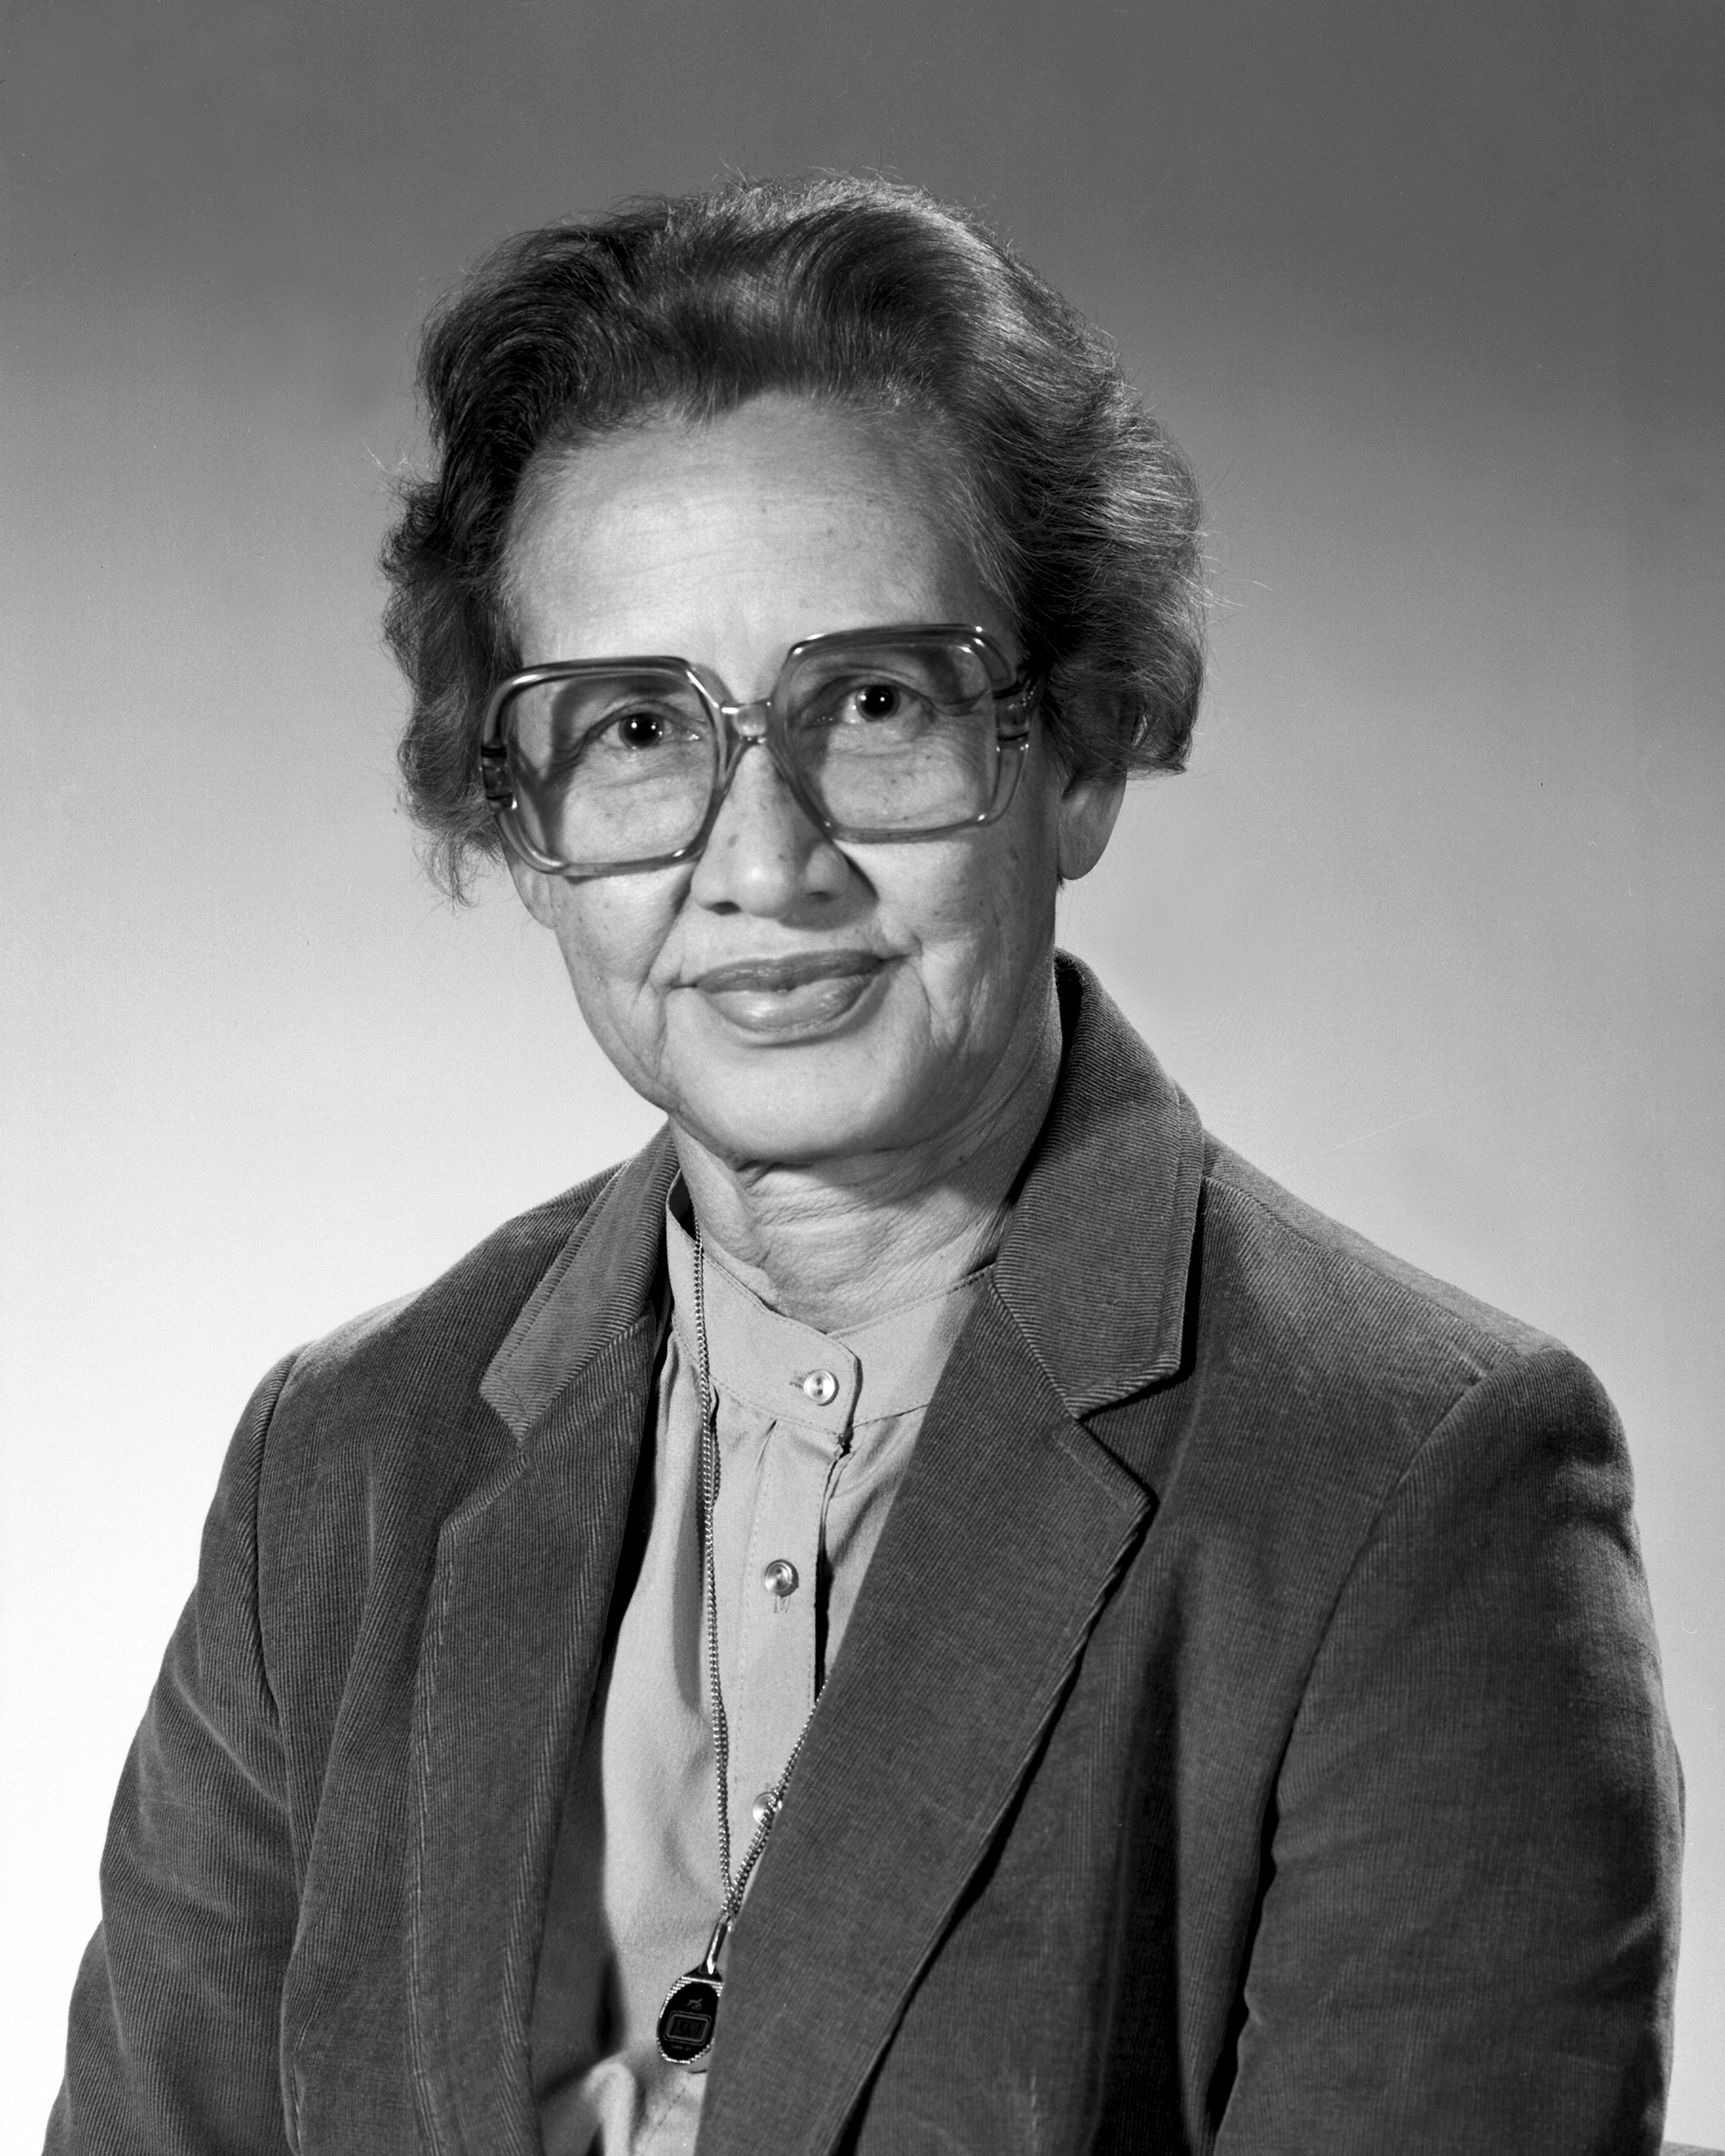
\includegraphics[height=2in]{katherine-johnson.jpeg}
  \end{center}
  % Margaret Hamilton: coding lead for Apollo project
  % Katherine Johnson: computer!  NASA. Hidden Figures.
\end{frame}

\begin{frame}{}
  \begin{center}
    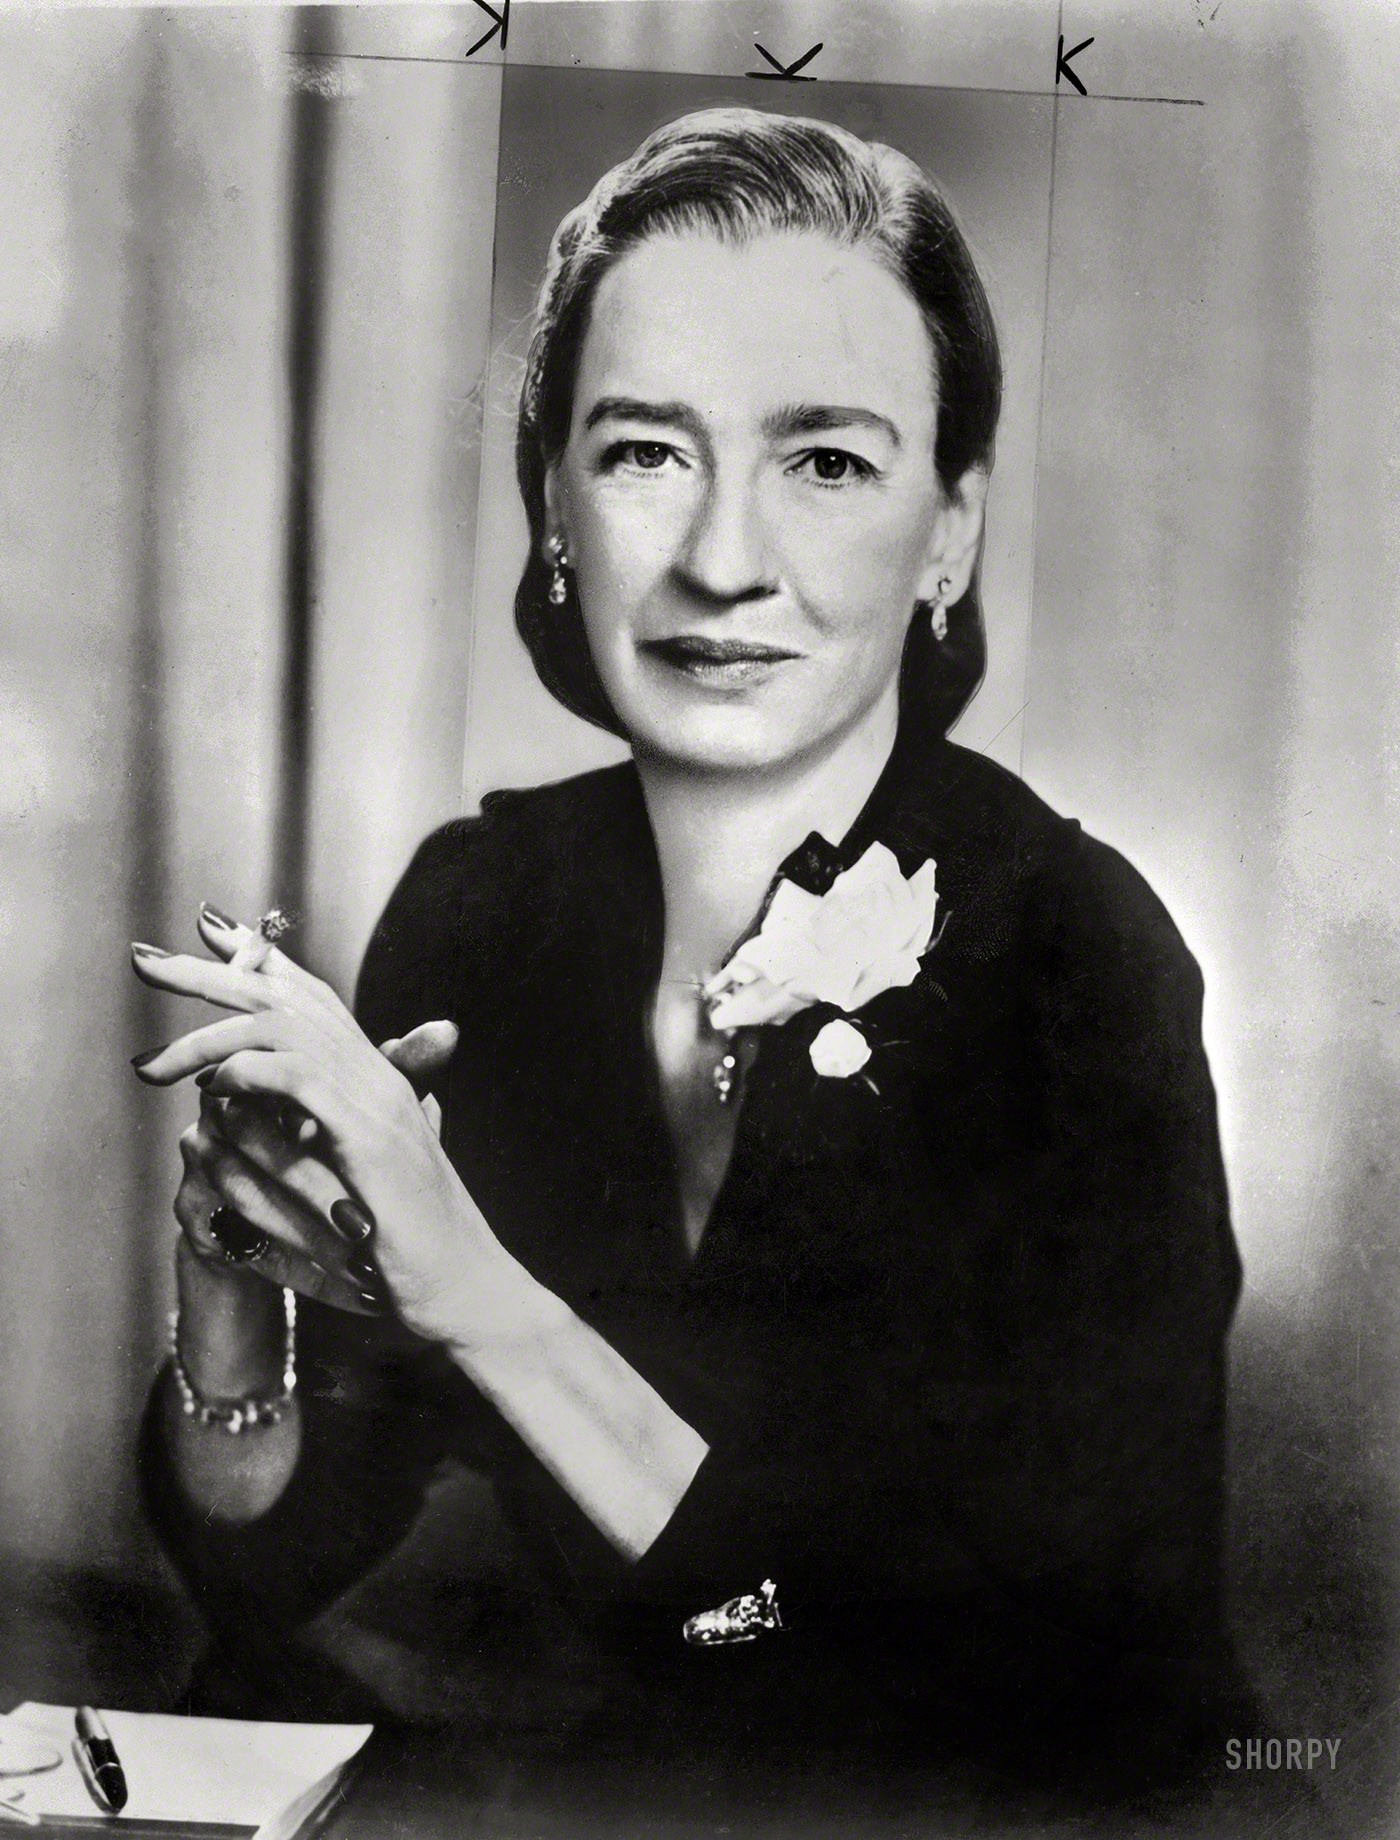
\includegraphics[height=2in]{grace-hopper.jpg} \quad
    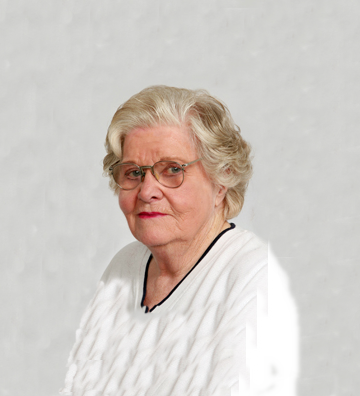
\includegraphics[height=2in]{jean-bartik-cropped.png}
  \end{center}
  % Grace Hopper
  % Jean Bartik: programmed ENIAC
\end{frame}

\end{document}
